\newpage 
\section{Future Plan}~\label{sec:discussion}
The future plan for this research is shown in Figure-\ref{fig:plan}. The main activities planned for this research are:
\begin{itemize}
    \item Development of a method for calculating the effect of an induced emotion on a conversation, using the empirical analysis of the first research question, as well as the findings in the literature, to develop a function for assigning weights to the various emotions in a social media conversation.
    \item Development of machine learning-based recommender system for context-based emotion regulation strategy recommendation for online conversations in order to provide on-the-spot ER support in instances of intensified emotional expression.
    \item Scientific papers and writing the thesis.
\end{itemize}
\begin{figure}[h]
  
    \centering
    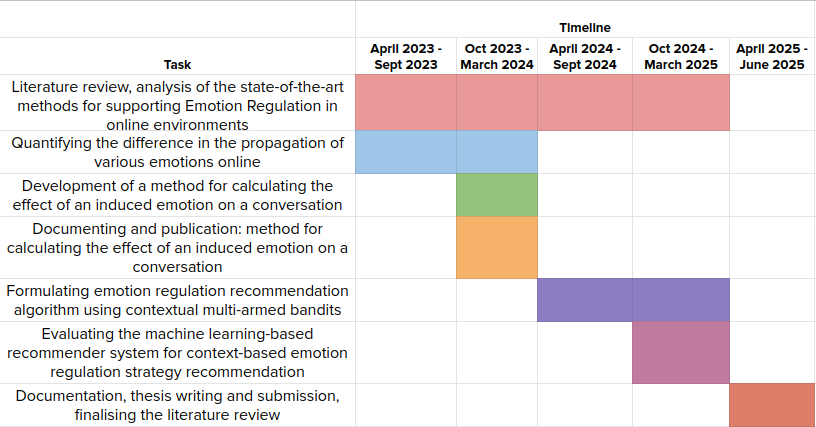
\includegraphics[width=14cm,height=14cm,keepaspectratio]{plan.png}
%   \includegraphics[width=5cm,height=5cm,keepaspectratio]{samples/sample_convv.png}
%   \includegraphics[width=5cm,height=5cm,keepaspectratio]{samples/sample_conv_graphh.png}
  \caption{Future Plan}
  \label{fig:plan}
  \end{figure} 

The remainder of the research strategy entails an ongoing literature review of state-of-the-art methods for supporting Emotion Regulation in online environments. The following phase contains quantifying the difference in the online propagation of various emotions, as well as developing a method for calculating the effect of an induced emotion on a conversation and documenting and publishing the same, between April 2023 and March 2024. Following that, it includes formulating emotion regulation recommendation algorithm using contextual multi-armed bandits and Evaluating the machine learning-based recommender system for context-based emotion regulation strategy recommendation as well as documentation, thesis writing and submission, and finalising the literature review between April 2024 and June 2025.
  
\subsection{List of Publications}
\begin{itemize}
    \item Encouraging Emotion Regulation in Social Media Conversations through Self-Reflection, \textit{preparing for submission}
    \item Digital Emotion Regulation on Social Media, \textit{preparing for submission}
\end{itemize}

